\documentclass{article}
\usepackage{stmaryrd}
\usepackage{graphicx}

\title{Report, Kinetic project}
\author{Dorian Geraldes Pereira, Axel Demuth}
\date{March 2024}

\begin{document}
\maketitle
\tableofcontents
\newpage


\section{Objectives}
To be able to solve equations on a mesh, we need it to be watertight.

The objectives of the project are:

\begin{itemize}
    \item Repair mesh to make them watertight
   

    \begin{itemize}
        \item watertight building model
        

        \item watertight urban model
    \end{itemize} 
\end{itemize} 

In our project we will have to use files in IFC format containing building meshes that are not watertight in an algorithm repairing
geometric error in a kinetic data structures. We will have to find a way to keep the label 
on the surfaces in the algorithm or relabel every surfaces at the end.
we can see here an example of what we will need to do:

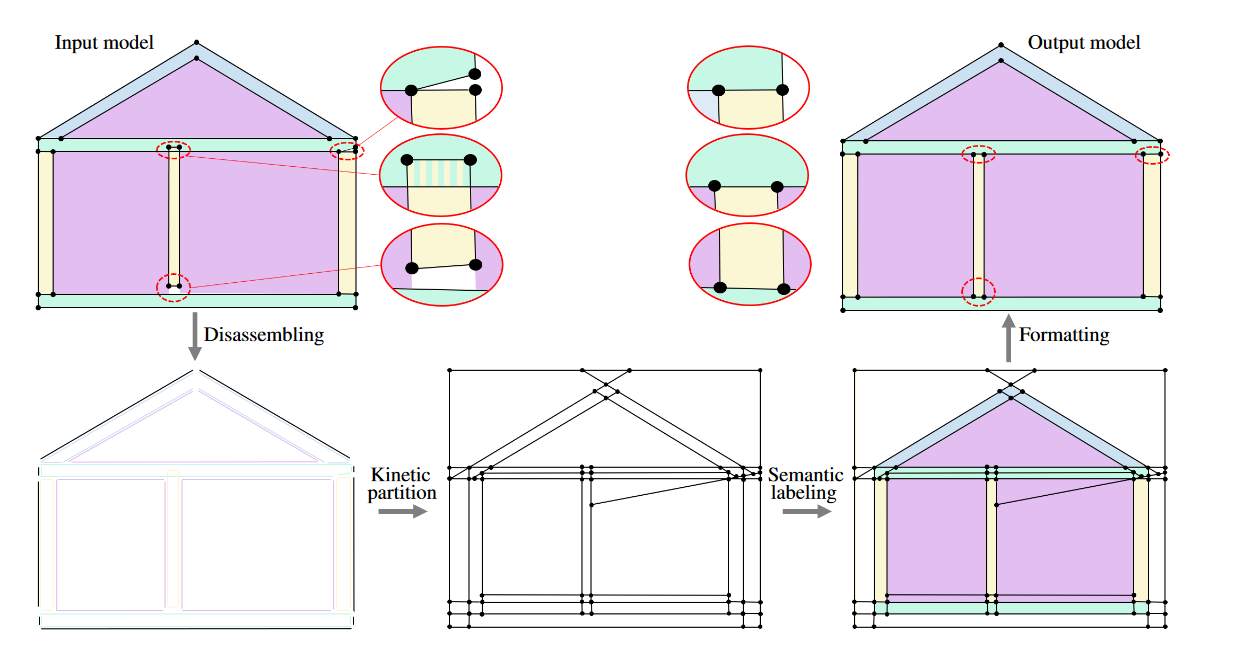
\includegraphics[scale = 0.37]{../images/example_algorithm_2.png}



\section{Tools}
\subsection{CGAL}
CGAL is a comprehensive package for geometry algorithms, providing various data structures and algorithms for working on polygons, surfaces, mesh generation, and more.
It offers a wide range of functionalities for geometric processing and analysis in various fields such as computer graphics, computational geometry, and geometric modeling.


\subsection{Kinetic}

Kinetic algorithms is a package from CGAL that allows working on meshes with some holes in them. When applied to the mesh, the Kinetic algorithms will 'extend' some surfaces to fill the mesh and make it watertight. 
Here's what the algorithm is capable of:

\begin{figure}[h]
    
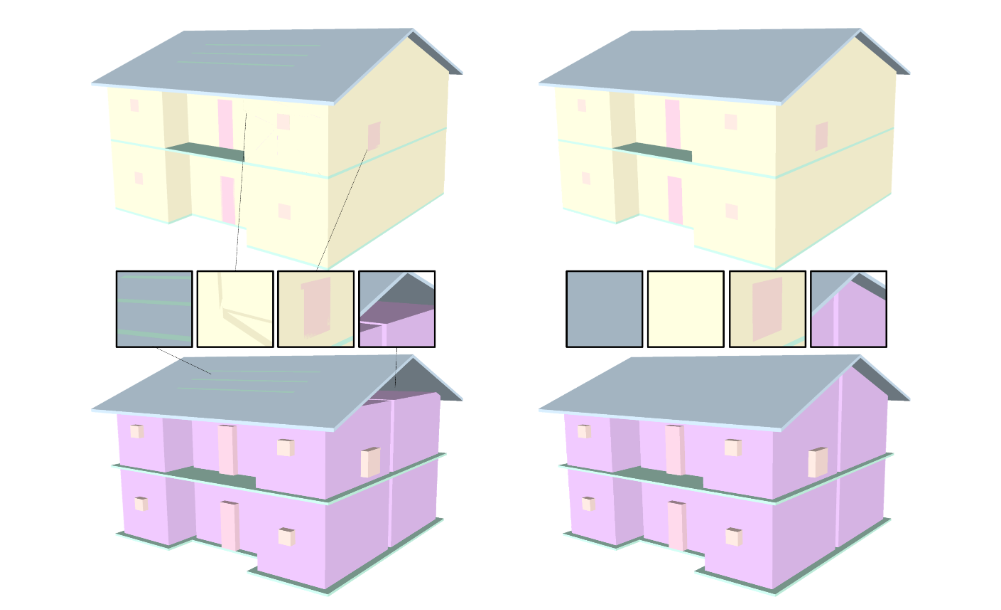
\includegraphics[scale =   0.3 ]{../images/example_algorithm.png}



\end{figure}

texte v1 : 
To use the algortihm we are using an algortihm from CGAL, when given a bunch of parameter and a files with a scatter plot and the normal associated to the point.
We had the chance to have a meeting with Florent Lafarge one of the creator of the algorithm,and he explain to us what parameter are important to analyse 
and which one gonna have a huge influence on the results.
There are 2 important parameter: distance and qmin here an example with both parameter varying:

\begin{figure}[h]
    \centering
    \begin{minipage}[b]{0.4\textwidth}
      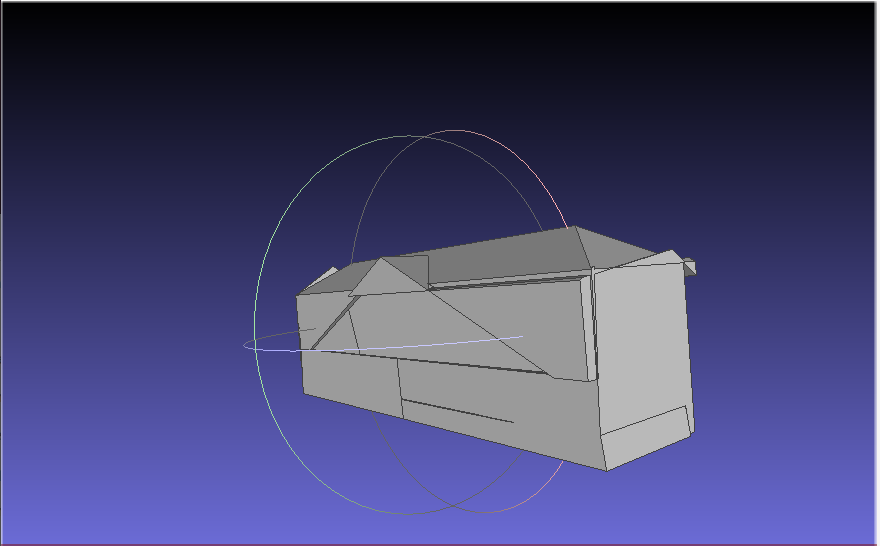
\includegraphics[width=\textwidth]{../images/screen_kinetic/dist1_pmin220.png}
      \caption{Image 1}
      \label{fig:image1}
    \end{minipage}
    \hfill
    \begin{minipage}[b]{0.4\textwidth}
      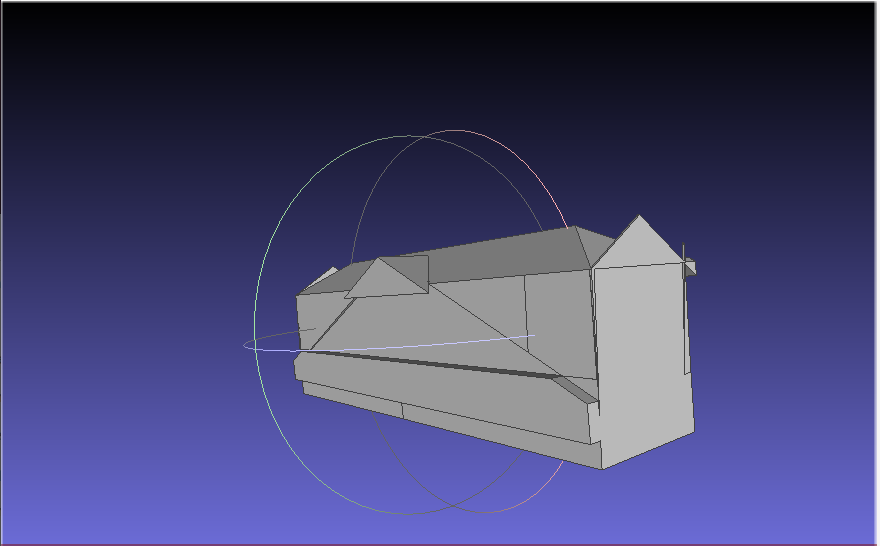
\includegraphics[width=\textwidth]{../images/screen_kinetic/dist1_pmin250.png}
      \caption{Image 2}
      \label{fig:image2}
    \end{minipage}
    \hfill
    \begin{minipage}[b]{0.4\textwidth}
      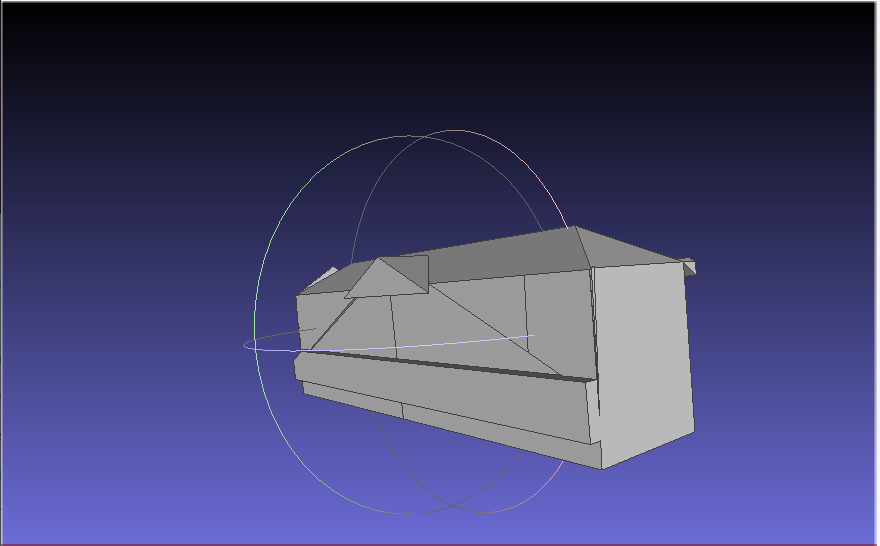
\includegraphics[width=\textwidth]{../images/screen_kinetic/dist1_pmin280.png}
      \caption{Image 3}
      \label{fig:image3}
    \end{minipage}
  \end{figure}
  
  \end{document}

include exemple de building avec les parametres qui varie 


One of the difficulty of studying this algorithm is judging the good qmin to get the good number of partition of the space, if u put it too big it will be more precise 
but it will take longer to  execute, and in some case bad values can make the program to crash.

(pas sur d'ecrire la phrase qui suit )
We could also take a look about the Kinetic Surface reperation Software from the INRIA titane team,to an easier application of scatter plot,With new function as refine the first partition to make it smoother or fitting better the geometric


(pourquoi on veut cet algo)
This algorithm could be a primordial tool in our project when having massive mesh for a huge building, an hospital,..., When we create huge mesh there can be some probleme in it, and for simulation this can be fatal error 
when trying to calculate something on the mesh leading to false result.With this algorithm allow us to fix the mesh.Another problem is the iput of the algorithm, only working for now ith scatter plot, so we cannot use the IFC format
loosing all information about what type of structures we have.To counter that we gonna try to do something like IFC --> scatterplot with data  -- > plt,ply,xyz.. format susported by kinetic CGAL and data  --> mesh with data 


\subsection{Roadmap}
We intend to work on this project in the coming months and will continuously update our progress as outlined in the following roadmap.
\begin{figure}[h]
    
    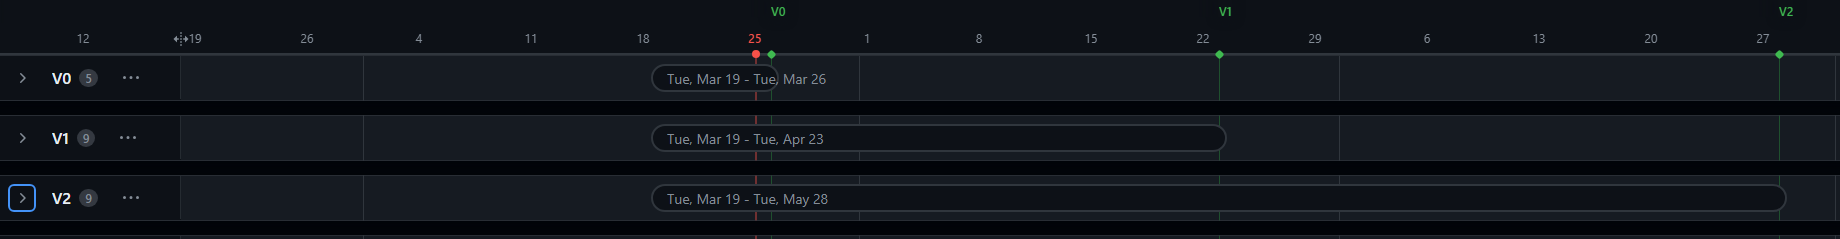
\includegraphics[scale =   0.3 ]{../images/roadmap.png}
    
\end{figure}
    
\nocite{*}
\bibliographystyle{plain}
\bibliography{../../bibliography/v0/report_bib}
\end{document}